\section{Introduction}
\label{sec:introduction}

In this project, I made a simple peg solitaire game using C++ with the \href{https://www.qt.io/}{Qt6 framework}.

\subsection{Main Objectives}
The primary aim of this project was to develop a fully functional and user-friendly Peg Solitaire game that provides an engaging puzzle-solving experience. The main objectives included:

\begin{itemize}
    \item Implementing the classic Peg Solitaire game mechanics with proper move validation and game rules
    \item Creating a clean, intuitive user interface that facilitates easy interaction
    \item Applying the Model-View-Controller (MVC) architecture to ensure maintainable and extensible code
    \item Providing different board layouts and game modes to enhance gameplay variety
    \item Implementing intelligent strategy features to assist players in finding solutions
    \item Ensuring cross-platform compatibility through the Qt6 framework
\end{itemize}

\subsection{Core Features}

\begin{figure*}[btp]
    \centering
    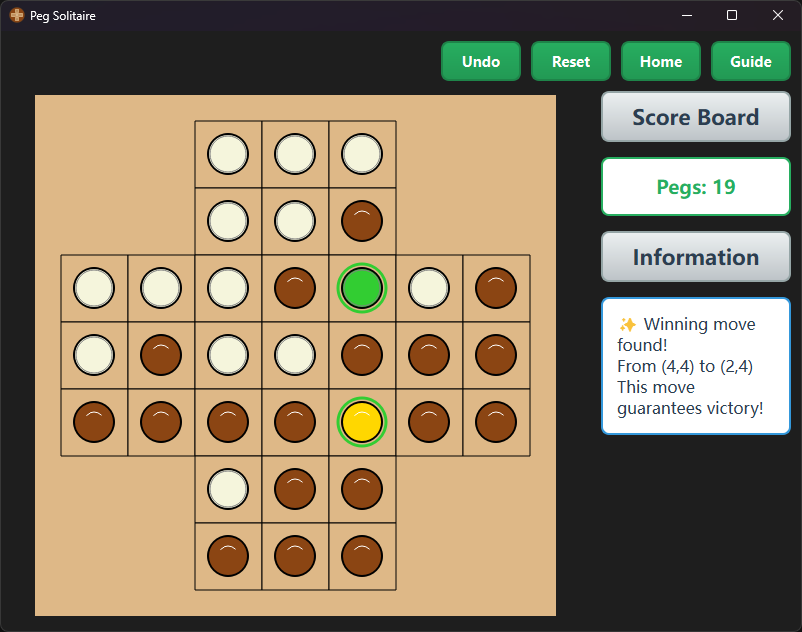
\includegraphics[width=0.3\textwidth]{resource/board-demos/EnglishBoard.png}
    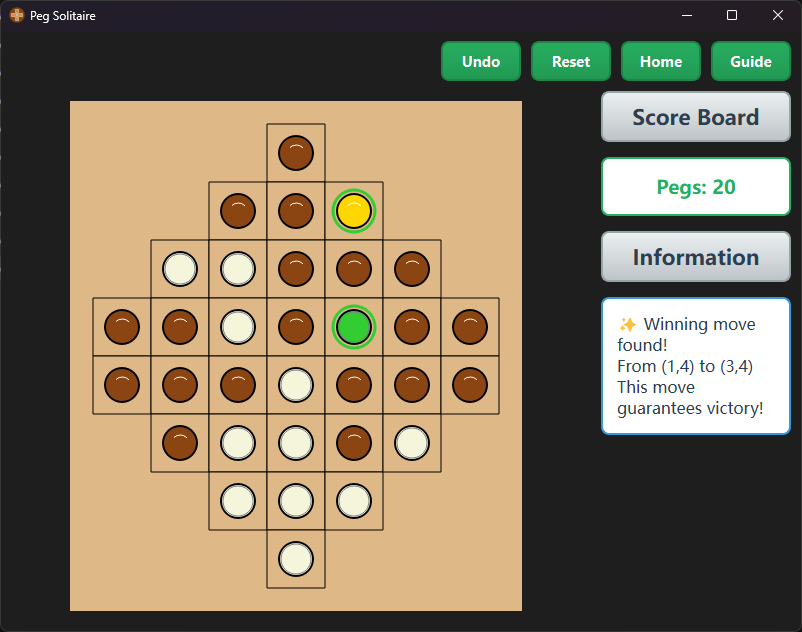
\includegraphics[width=0.3\textwidth]{resource/board-demos/DiamondBoard.png}
    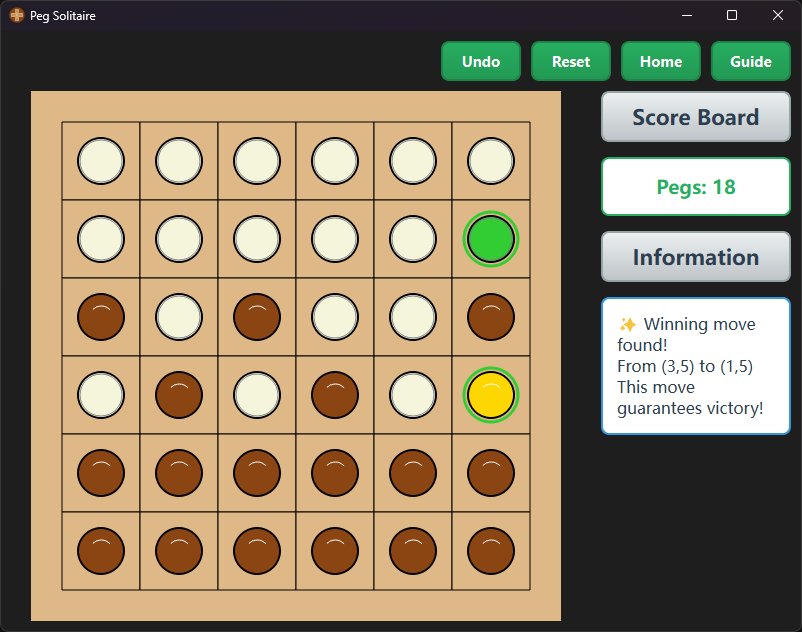
\includegraphics[width=0.3\textwidth]{resource/board-demos/SquareBoard.png}
    \caption{Different Peg Solitaire Board Layouts: English, Diamond, and Square}
    \label{fig:english-board}
\end{figure*}

The game includes a comprehensive set of core features that form the foundation of the gameplay experience:

\begin{figure*}[btp]
    \centering
    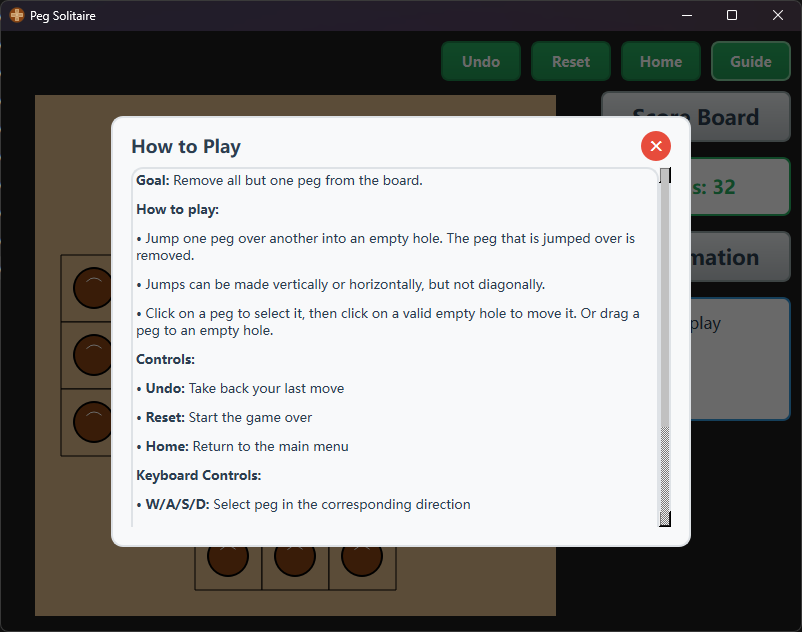
\includegraphics[width=0.5\textwidth]{resource/Guide.png}
    \caption{User Guide: How to Play Peg Solitaire}
    \label{fig:user-guide}
\end{figure*}

\begin{itemize}
    \item \textbf{Multiple Board Layouts}:
    The game offers several classic board layouts as is shown in Figure \ref{fig:english-board}, including:
    \begin{itemize}
        \item English (traditional 33-hole cross-shaped board)
        \item Diamond (diamond-shaped board)
        \item Square (square grid-based board)
    \end{itemize}
    
    \item \textbf{Intuitive Controls}: Players can interact with the game using:
    \begin{itemize}
        \item Mouse input for selecting and moving pegs
        \item Keyboard controls (WASD for peg selection, arrow keys for movement)
    \end{itemize}
    
    \item \textbf{Game Mechanics}: Fully implemented game mechanics including:
    \begin{itemize}
        \item Valid move detection and highlighting
        \item Win and lose condition detection
        \item Undo functionality for taking back moves
        \item Reset option to restart the current board
    \end{itemize}
    
    \item \textbf{User Interface}: A responsive UI with:
    \begin{itemize}
        \item HomePage with navigation options
        \item Game mode selection screen
        \item Settings page for game preferences
        \item In-game score tracking (remaining pegs counter)
        \item Information display showing current game status
    \end{itemize}

    \item \textbf{User Guide}: A comprehensive user guide is shown in Figure \ref{fig:user-guide}, which provides:
    \begin{itemize}
        \item The goal of the game, \emph{i.e.}, how to win the game
        \item How to play the game, including rules and valid moves
        \item Valid control operations, including \emph{undo}, \emph{reset}, and \emph{home} options
        \item How to use keyboard controls for peg selection and movement
        \item Tips on strategies for solving puzzles: try to work towards the center, avoid leaving isolated pegs, and focus on clearing edges first
    \end{itemize}
\end{itemize}

\subsection{Bonus Features}

\begin{figure*}[tbp]
    \centering
    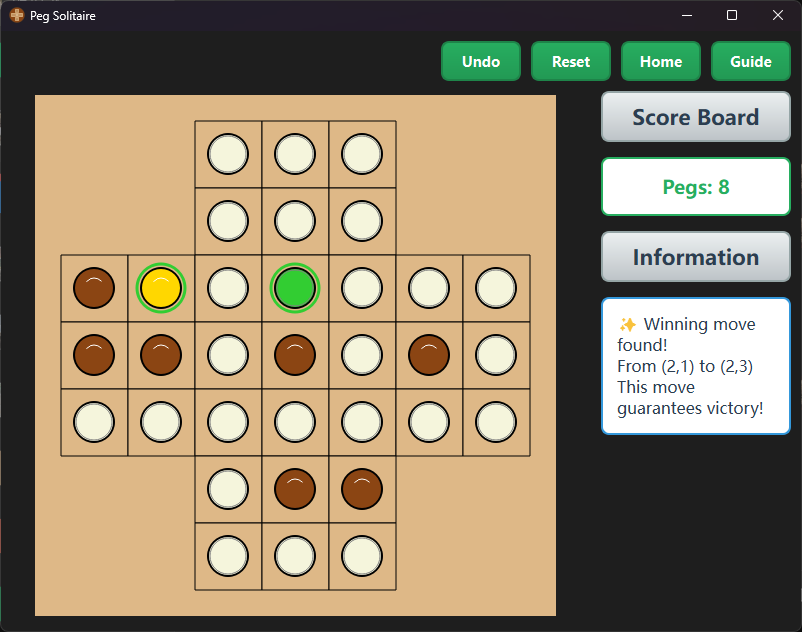
\includegraphics[width=0.3\textwidth]{resource/board-demos/AntiPegBoard.png}
    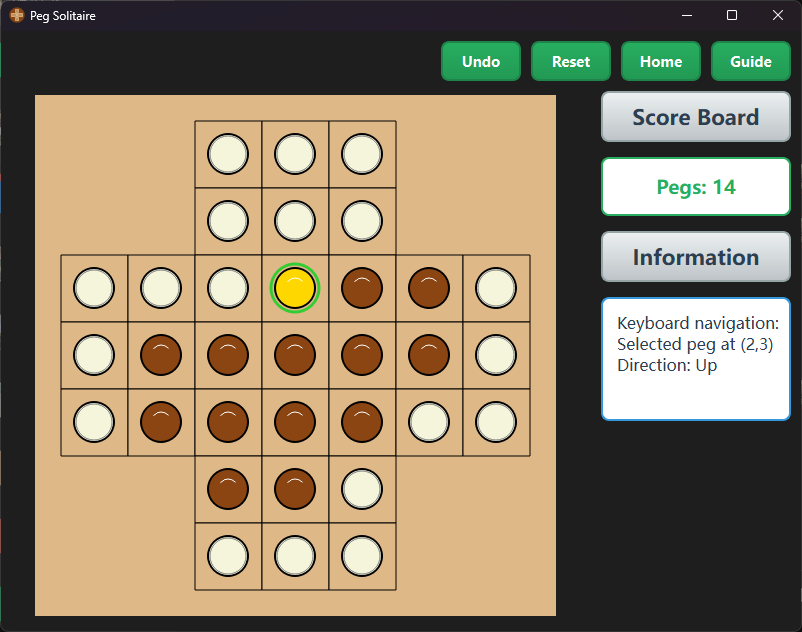
\includegraphics[width=0.3\textwidth]{resource/board-demos/EndgameBoard.png}
    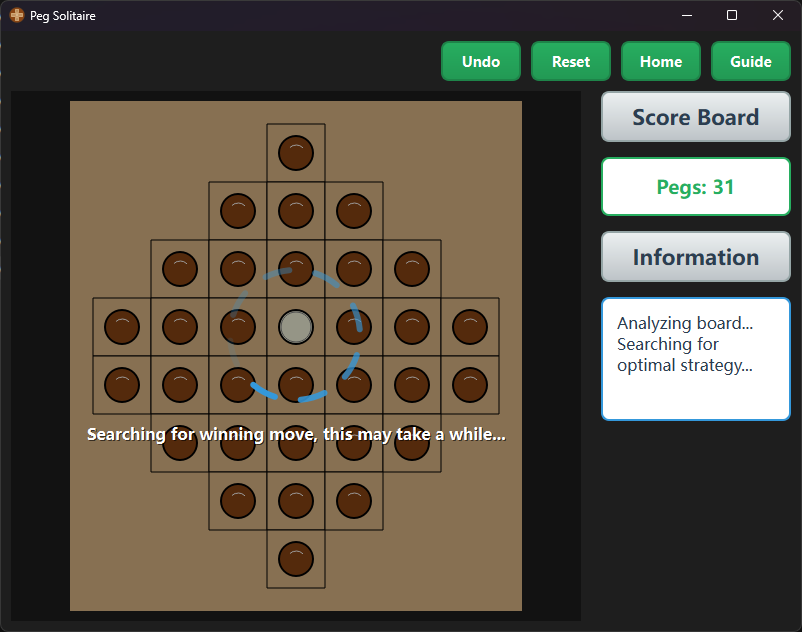
\includegraphics[width=0.3\textwidth]{resource/StrategyAssistant.png}
    \caption{Bonus Features: Anti-Peg Mode, Endgame Mode, and Strategy Assistant}
    \label{fig:bonus-features}
\end{figure*}

Beyond the core gameplay mechanics, I implemented several innovative features to enhance the player experience:

\begin{itemize}
    \item \textbf{Special Game Modes}:
    Figure \ref{fig:bonus-features} illustrates two unique game modes that provide fresh challenges:
    \begin{itemize}
        \item \textbf{Anti-Peg Mode}: An inverse version of the classic game where players start with a single peg and aim to fill the board by jumping pegs over empty spaces. The move mechanics are reversed, requiring a completely different strategy.
        
        \item \textbf{Endgame Mode}: Randomly generated but guaranteed-solvable puzzle configurations that challenge players with mid-game scenarios. These puzzles are created by working backward from a winning position, ensuring they always have at least one solution.
    \end{itemize}
    
    \item \textbf{Strategy Assistant}:
    \begin{itemize}
        \item Players can press the Spacebar to receive move suggestions.
        \item The system uses depth-first search (DFS) to determine if the current board state is winnable.
        \item Visual feedback through a loading animation indicates when the strategy calculation is in progress.
        \item Dead-game detection alerts players when no winning solution exists from the current position.
    \end{itemize}
    
    \item \textbf{Technical Optimizations}:
    \begin{itemize}
        \item Board symmetry recognition to optimize the solution-finding algorithm
        \item Multithreaded strategy computation to maintain UI responsiveness
        \item Dynamic sizing and responsive layout for different screen resolutions
        \item Fullscreen mode option for an immersive gaming experience
    \end{itemize}
\end{itemize}